%% Journal of Open Research Software Latex template -- Created By Stephen Bonner and John Brennan, Durham Universtiy, UK.

\documentclass{jors}

%  packages used by the xarray paper
\usepackage{natbib}
\usepackage{graphicx}
\usepackage{url}
\graphicspath{ {figures/} }
\setlength{\parskip}{1em}
% port install texlive-bibtex-extra
% port install texlive-bin texlive-bin-extra

%% Set the header information
\pagestyle{fancy}
\definecolor{mygray}{gray}{0.6}
\renewcommand\headrule{}
\rhead{\footnotesize 3}
\rhead{\textcolor{gray}{xarray: N-D labeled arrays and datasets in Python}}

\begin{document}

{\bf Software paper for submission to the Journal of Open Research Software} \\

% To complete this template, please replace the blue text with your own. The paper has three main sections: (1) Overview; (2) Availability; (3) Reuse potential. \\
%
% Please submit the completed paper to: editor.jors@ubiquitypress.com
\bibliographystyle{abbrv}

\rule{\textwidth}{1pt}

\vspace{0.5cm}

\section*{Title}

xarray: N-D labeled arrays and datasets in Python

\section*{Paper Authors}

{1. Hoyer, Stephan \\
 2. Hamman, Joseph J.}

\section*{Paper Author Roles and Affiliations}
{1. The Climate Corporation, San Francisco, CA, USA and Google Research, Mountain View, CA, USA. Present address: Google Research. 2. Department of Civil \& Environmental Engineering, University of Washington, Seattle, WA, USA.}

\section*{Abstract}

\textbf{xarray} is an open source project and Python package that provides a toolkit and data structures for N-dimensional labeled arrays.
Our approach combines an API inspired by pandas with the Common Data Model for self-described scientific data.
Key features of the \textbf{xarray} package include label-based indexing and arithmetic, interoperability with the core scientific Python packages (e.g., Pandas, NumPy, Matplotlib), out-of-core computation on datasets that don't fit into memory, a wide range of serialization and input/output (I/O) options, and advanced multi-dimensional data manipulation tools such as group-by and resampling.

\textbf{xarray}

\section*{Keywords}

{Data Analysis; Python; pandas; netCDF}

\section*{(1) Overview}

\section*{Introduction}

Python has emerged as a leading programing language for both the physical sciences and data sciences.
At the core of modern scientific computing and analysis in Python are the NumPy \citep{Jones_2001} and SciPy \citep{van_der_Walt_2011} packages, which provide a robust N-dimensional array object and the fundamental operations required for science and engineering applications.
Much of the success of Python in data science and business analytics is due to pandas \citep{mckinney_2010}, which introduced intuitive and fast tabular data analysis tools to Python, inspired by R's \verb|data.frame| \citep{r_2013}.
The pandas \verb|DataFrame| and \verb|Series| objects provide unparalleled analysis tools for data alignment, resampling, grouping, pivoting, and aggregation.

\textbf{xarray} implements data structures and an analytics toolkit for multi-dimensional
labeled arrays strongly inspired by pandas.
While pandas includes a data structure called the \verb|Panel| for three dimensional data, its fixed rank design make it unsuitable for applications that require arbitrary rank arrays.
Our approach with \textbf{xarray} adopts the self-describing Common Data Model on which the network Common Data Form (netCDF) is built \citep{Rew_1990,Brown_1993}.
NetCDF provides a well-defined data model for labeled N-dimensional array-oriented scientific data analysis.

\textbf{xarray} builds on top of, and seamlessly interoperates with, the core scientific Python packages, such as NumPy, SciPy, Matplotlib \citep{Hunter_2007}, and pandas.
\textbf{xarray} provides a range of backends for serialization and input/output (IO), including the Pickle, netCDF, OPeNDAP (read-only), GRIB1/2 (read-only), and HDF file formats.
Leveraging the dask parallel computing library, \textbf{xarray} can optionally perform efficient parallel, out-of-core analysis on datasets that are too large to fit into memory.
Finally, \textbf{xarray} interfaces with existing domain-specific packages such as UV-CDAT \citep{uvcdat}, Iris \citep{Iris}, and Cartopy \citep{Cartopy}.

\begin{figure}[h]
	\centering
	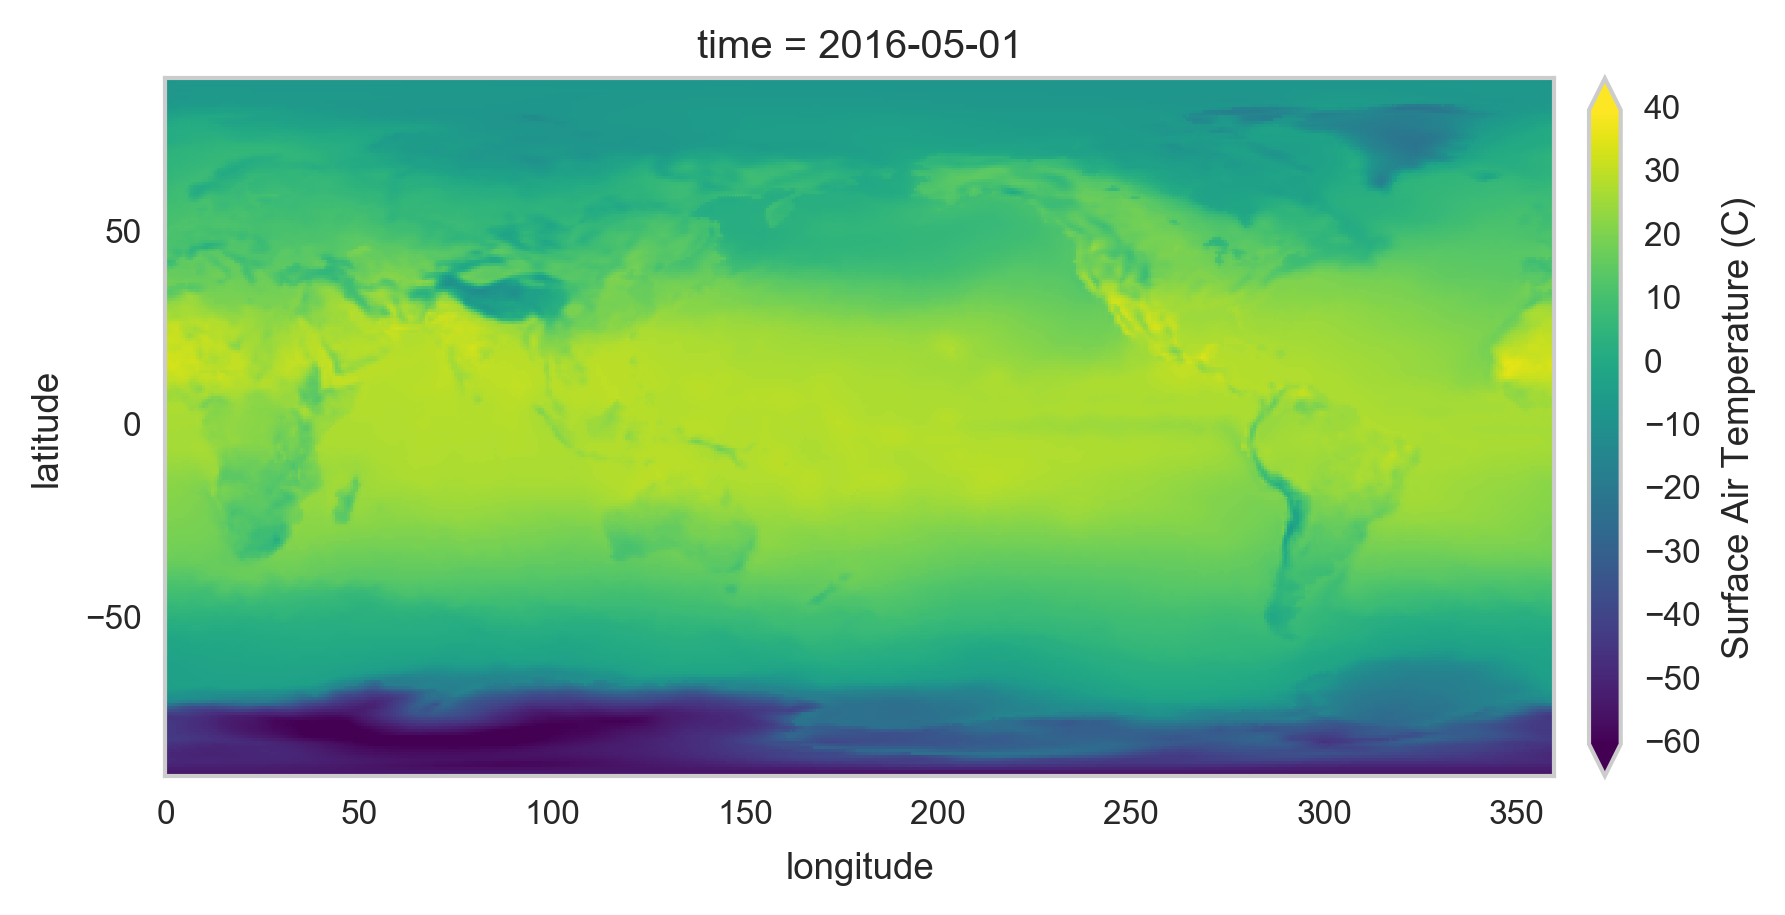
\includegraphics[width=0.8\textwidth]{ERA-Interim_surface_air_temp_figure}
	\caption{An example of a multidimensional labeled array. This figure (map) is showing the global surface air temperature for May 1, 2016 from ERA-Interim Reanalyis \citep{Dee_2011}. The map is labeled with the array's coordinates: longitude and latitude.}
	\label{fig:temperature_map}
\end{figure}

\textbf{Purpose: Your data has labels; you should use them}

Scientific data is inherently labeled.
For example, time series data includes time\-stamps that label individual periods or points in time, spatial data has coordinates (e.g. longitude, latitude, elevation), and model or laboratory experiments are often identified by unique identifiers.
Figure \ref{fig:temperature_map} provides an example of a labeled dataset.
In this case the data is a map of global air temperature from a numeric weather model.
The labels on this particular dataset are time (e.g. ``2016-05-01''), longitude (x-axis), and latitude (y-axis).

Unlabeled, N-dimensional arrays of numbers, implemented in the SciPy ecosystem by NumPy, are the most widely used data structure in Python's scientific computing ecosystem.
However, they lack a meaningful representation of the metadata associated with their data.
Implementing such functionality is left to individual users and domain-specific packages.
As a result, data scientists frequently encounter pitfalls in the form of questions like ``is the time axis of my array in the first or third index position?'' or ``does my array of timestamps still align with my data after resampling?''.

The core motivation for developing \textbf{xarray} was to provide labeled data tools for N-dimensional arrays that render such questions moot. Every operation in xarray both relies on and maintains the consistency of labels.

\textbf{NetCDF}

The network Common Data Form is a collection of self-describing, machine-independent binary data formats and software tools.
These data formats and tools facilitate the creation, access, and sharing of scientific data stored in N-dimensional arrays, along with metadata describing the contents of each array \citep{Rew_1990}.
NetCDF has become very popular in the geoscience community, and there are existing libraries for reading and writing netCDF in many programming languages, including C, Fortran, Python, Java, Matlab, and Julia.

The principal data structure in the netCDF data model is the \verb|dataset|.
Each netCDF \verb|dataset| contains \verb|dimensions|, \verb|variables|, and \verb|attributes|, each of which are identified by a hierarchy of unique names.
The \verb|dataset| and \verb|variable| objects may contain \verb|attributes| that describe the contents, units, history, or other metadata of the object.
Standardized conventions, such as the Climate and Forecast (CF) Conventions \citep{eaton2003netcdf}, allow for the associations of coordinate variables with \verb|dimensions|.

\section*{Implementation and architecture}

NetCDF forms the basis of the \textbf{xarray} data model and provides a natural and portable serialization format.
\textbf{xarray} provides two main data structures the \verb|DataArray| and the \verb|Dataset|.

\begin{figure}
	\centering
	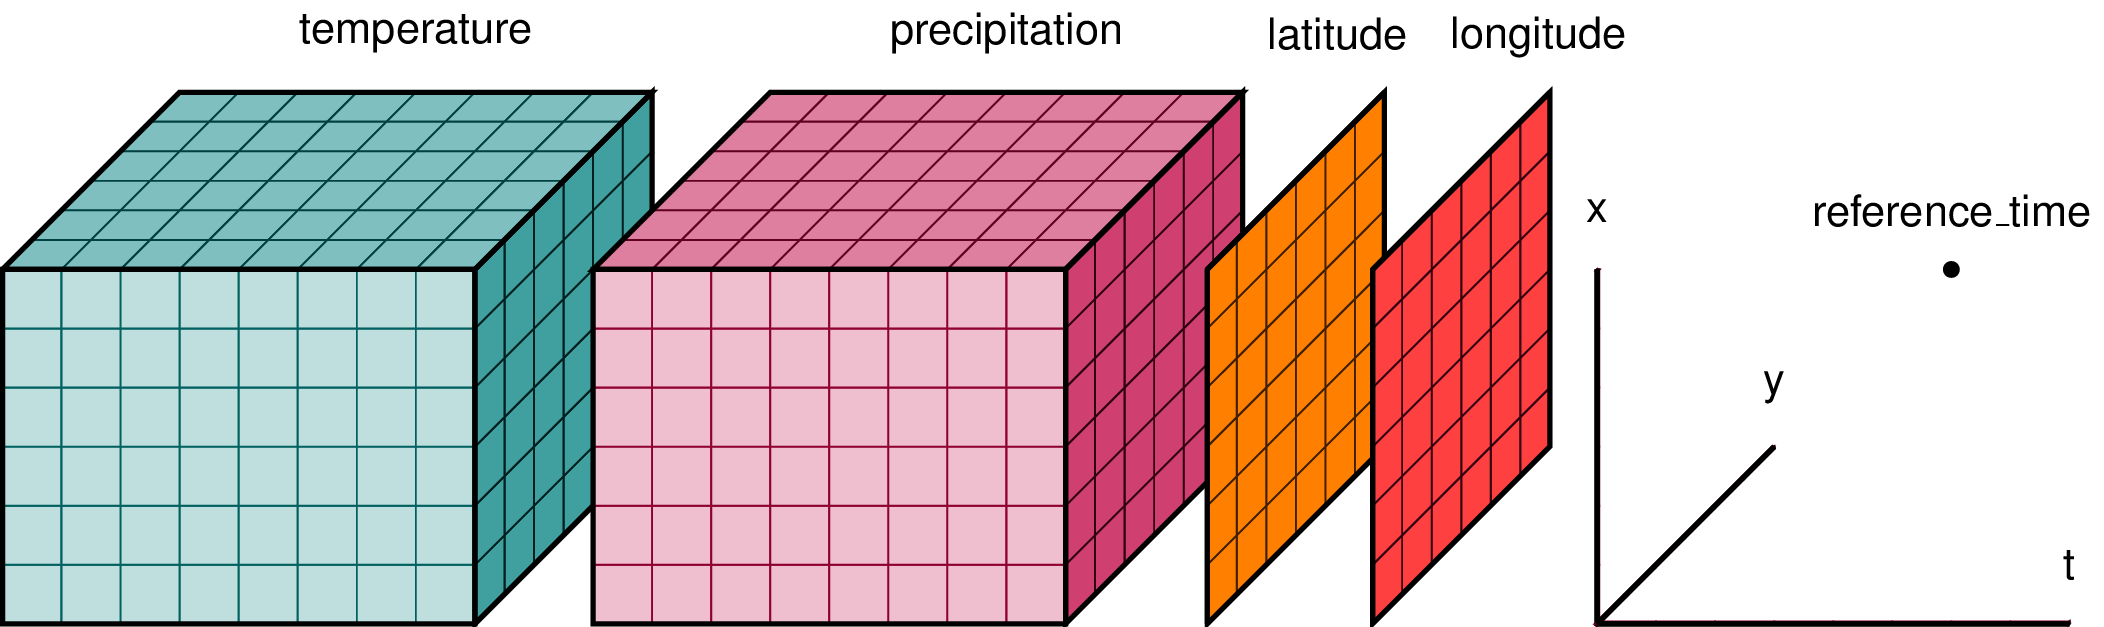
\includegraphics[width=0.8\textwidth]{dataset-diagram_original}
	\caption{An example of how a dataset (netCDF or \textbf{xarray}) for a weather forecast might be structured. This dataset has three dimensions, time, y, and x, each of which is also a one-dimensional coordinate. \textit{Temperature} and \textit{precipitation} are three-dimensional data variables.  Also included in the dataset are two-dimensional coordinates \textit{latitude} and \textit{longitude}, having dimensions y and x, and \textit{reference time}, a zero-dimensional (scalar) coordinate.}
	\label{fig:dataset_diagram}
\end{figure}

\textbf{DataArray}

The \verb|DataArray| is \textbf{xarray's} implementation of a labeled, multi-dimensional array. It has several key properties:

\begin{itemize}
	\item \verb|data|: N-dimensional array (NumPy or dask) holding the array's values,
	\item \verb|dims|: dimension names for each axis [e.g., \verb|(`time', `latitude', `longitude')|],
	\item \verb|coords|: dict-like container of arrays (coordinates) that label each point (e.g., 1-dimensional arrays of numbers, \verb|datetime| objects or strings), and
	\item \verb|attrs|: \verb|OrderedDict| holding arbitrary metadata (e.g. units or descriptions)
\end{itemize}

\textbf{xarray} uses \verb|dims| and \verb|coords| to enable its core metadata-aware operations.
Dimensions provide names that \textbf{xarray} uses instead of the axis argument found in many NumPy functions.
Coordinates are ancillary variables used to enable fast label-based indexing and alignment, building on the functionality of the pandas \verb|Index|.
\verb|DataArray| objects also can have a name and can hold arbitrary metadata in the form of their \verb|attrs| property, which can be used to further describe data (e.g. by providing units).
Names and attributes are strictly for users and user-written code; in general \textbf{xarray} makes no attempt to interpret them, and propagates them only in unambiguous cases.
In contrast, \textbf{xarray} does interpret and persist coordinates in operations that transform \textbf{xarray} objects.

\textbf{Dataset}

The \verb|Dataset| is \textbf{xarray's} multi-dimensional equivalent of a \verb|DataFrame|. It is a dict-like container of labeled arrays (\verb|DataArray|s) with aligned dimensions.
It is designed as an in-memory representation of a netCDF dataset.
In addition to the dict-like interface of the dataset itself, which can be used to access any \verb|DataArray| in a \verb|Dataset|, datasets have four key properties:

\begin{itemize}
	\item \verb|dims|: dictionary mapping from dimension names to the fixed length of each dimension (e.g., \verb|{`x': 6, `y': 6, `time': 8}|)
	\item \verb|data vars|: dict-like container of \verb|DataArray|s corresponding to data variables
	\item \verb|coords|: dict-like container of \verb|DataArray|s intended to label points used in \verb|data vars| (e.g., 1-dimensional arrays of numbers, \verb|datetime| objects or strings)
	\item \verb|attrs|: \verb|OrderedDict| to hold arbitrary metadata pertaining to the dataset
\end{itemize}

\verb|DataArray|s can share any number of common dimensions common, but they are presumed to share a common coordinate system.
Coordinates can also have any number of dimensions but denote constant/independent quantities, unlike the varying/dependent quantities that belong in data.
Figure \ref{fig:dataset_diagram} illustrates these concepts for an example \verb|Dataset| containing meteorological data.

\textbf{Core xarray Features}

\textbf{xarray} includes a powerful and growing feature set.
The following list highlights some of the key features available in \textbf{xarray}.
The xarray documentation \citep{xarray_docs} includes a complete description of available features and their usage.

\begin{itemize}
	\item \textit{Label-based indexing}: Similarly to pandas objects, \textbf{xarray} objects support both integer- and label-based lookups along each dimension.
	However, \textbf{xarray} objects also have named dimensions, so you can optionally use dimension names instead of relying on the positional ordering of dimensions.
	\item \textit{Arithmetic}: arithmetic between \textbf{xarray} objects vectorizes based on dimension names, automatically looping (broadcasting) over each distinct dimension.
	\item \textit{Aggregation}: calculation of statistics (e.g. sum) along a dimension of an \textbf{xarray} object can be done by dimension name instead of an integer axis number.
	\item \textit{Alignment}: \textbf{xarray} features database-like alignment based on coordinate labels that smoothly handles missing values.
	\item \textit{Split-apply-combine}: \textbf{xarray} includes N-dimensional grouped operations implementing the split-apply-combine strategy \citep{wickham_2011}.
	\item \textit{Resampling and rolling window operations}: Utilizing the efficient resampling methods from pandas and rolling window operations from Bottleneck \citep{Bottleneck}, \textbf{xarray} offers a robust set of resampling and rolling window operations along a single dimension.
	\item \textit{Plotting}: \textbf{xarray} plotting functionality is a thin wrapper around the popular Matplotlib library.
	\textbf{xarray} uses the syntax and function names from Matplotlib whenever possible, resulting in a seamless transition between the two.
	\item \textit{Interactivity with pandas}: \textbf{xarray} objects seamlessly to convert to and from pandas objects to interact with the rest of the PyData ecosystem.
	\item \textit{Serialization and I/O}: \textbf{xarray} supports direct serialization and I/O to several file formats including pickle, netCDF, OPeNDAP (read-only), GRIB1/2 (read-only), and HDF by integrating with third-party libraries.
	Additional serialization formats for 1-dimensional data are available through pandas.
	\item \textit{Out-of-core computation}: \textbf{xarray} integrates with dask to support parallel and streaming computation on datasets that do not fit into memory.
\end{itemize}

\section*{Quality control}

% \textcolor{blue}{Detail the level of testing that has been carried out on the code (e.g. unit, functional, load etc.), and in which environments.
% If not already included in the software documentation, provide details of how a user could quickly understand if the software is working (e.g. providing examples of running the software with sample input and output data). }

\textbf{xarray} is provided with a large test suite comprised of over 950 unit tests.
These tests cover the core \textbf{xarray} functionality as well as features facilitated by optional dependencies.
The unit tests are executed automatically on the TravisCI (Linux) \citep{TravisCI} and Appveyor (Windows) \citep{Appveyor} continuous integration systems.
A selection of sample data is also distributed with the source code, allowing users to reproduce any examples in the \textbf{xarray} documentation.

\section*{(2) Availability}
\vspace{0.5cm}
\section*{Operating system}

Linux, Windows and Mac OS X.

\section*{Programming language}

Python, versions 2.7, 3.3 and later.

\section*{Additional system requirements}

None.

\section*{Dependencies}

\textbf{xarray} is implemented in pure Python and relies on compiled dependencies for
speed.

\begin{itemize}
\item NumPy: 1.7 or later
\item pandas: 0.15.0 or later
\item netcdf4-python: (optional) used for reading and writing netCDF files
\item SciPy: (optional) used as a fallback for reading/writing netCDF3
\item Pydap: (optional) used as a fallback for accessing OPeNDAP
\item h5netcdf: (optional) an alternative library for reading and writing netCDF4 files that does not use the netCDF-C libraries
\item PyNIO: (optional) for reading GRIB1/2 and other geoscience specific file formats
\item Bottleneck: (optional) speeds up NaN-skipping and rolling window aggregations by a large factor
\item cyordereddict: (optional) speeds up most internal operations with \textbf{xarray} data structures
\item Dask: (optional) required for out-of-core parallel computation
\item Matplotlib: (optional) required for plotting
\item Cartopy: (optional) required for plotting maps
\item seaborn: (optional) additional plotting functionality
\end{itemize}

\section*{List of contributors}

\begin{itemize}
\item Alex Kleeman, The Climate Corporation
\item Alistair Miles, Wellcome Trust Centre for Human Genetics, University of Oxford
\item Andreas Hilboll, Institute of Environmental Physics, University of Bremen
\item Anna Kuznetsova, The Climate Corporation
\item Antony Lee, Department of Physics, University of California, Berkeley
\item Benjamin Root, Atmospheric and Environmental Research, Inc.
\item Benoit Bovy, Department of Astrophysics, Geophysics and Oceanography, University of Liège
\item Christoph Deil, Max Planck Institute for Nuclear Physics
\item Clark Fitzgerald, Department of Statistics, University of California, Davis
\item Dean Pospisil, Institute for Learning and Brain Sciences, University of Washington
\item Edward Richards, Scripps Institution of Oceanography, University of California, San Diego
\item Erik Welch, Continuum Analytics
\item Eugene Brevdo, Google Research
\item Fabien Maussion, Institute of Atmospheric and Cryospheric Sciences, University of Innsbruck
\item Filipe Fernandes, Universidade de São Paulo
\item Igor Babuschkin, School of Physics and Astronomy, University of Manchester
\item Jeffrey Gerard, The Climate Corporation
\item Jeremy McGibbon, Department of Atmospheric Sciences, University of Washington
\item Joseph Hamman, Civil and Environmental Engineering, University of Washington
\item Jonathan Helmus, Environmental Science Division, Argonne National Laboratory
\item Kelsey Jordahl, Planet Labs
\item Maciek Swat, University of Pennsylvania
\item Markel García-Díez, Catalan Institute of Climate Sciences
\item Maximilian Roos, Sixty Capital
\item Mike Graham, Edgestream Partners
\item Nikolay Koldunov, Climate Service Center Germany
\item Peter Cable, Raytheon
\item Phillip J. Wolfram, Fluid and Solid Mechanics (T-3), Theoretical Division, Los Alamos National Laboratory
\item Rafael Guedes, MetOcean Solutions Ltd
\item Ryan Abernathey, Department of Earth and Environmental Sciences, Columbia University
\item Scott Sinclair, Satellite Applications and Hydrology Group, Dept. Civil Engineering, University of KwaZulu-Natal
\item Sébastien Celles, Thermal Science and Energy Department, Poitiers Institute of Technology (IUT)
\item Spencer A. Hill, Program in Atmospheric and Oceanic Sciences, Princeton University
\item Stefan Pfenninger, Department of Environmental Systems Science, ETH Zürich
\item Stephan Hoyer, Google Research
\item Steven E. Pav, Gilgamath Consulting
\item Takeshi Kanmae, National Institute of Polar Research
\item Thomas Kluyver, Computational Modelling Group, University of Southampton
\item Todd Small, The Climate Corporation
\item Valliappa Lakshmanan, Google
\end{itemize}

\section*{Software location:}

{\bf Archive}

\begin{description}[noitemsep,topsep=0pt]
	\item[Name:] Zenodo
	\item[Persistent identifier:] \url{http://dx.doi.org/10.5281/zenodo.59499}
	\item[Licence:] Apache, v2.0
	\item[Publisher:]  Zenodo
	\item[Version published:] 0.8.2
	\item[Date published:] August 18, 2016
\end{description}

{\bf Code repository}

\begin{description}[noitemsep,topsep=0pt]
	\item[Name:] GitHub
	\item[Identifier:] \url{http://github.com/pydata/xarray}
	\item[Licence:] Apache, v2.0
	\item[Date published:] August 18, 2016
\end{description}

\section*{Language}

English.

\section*{(3) Reuse potential}

\textbf{xarray} was written in a modular, objected-oriented way, to build upon and extend the core scientific Python libraries in a domain-agnostic fashion.
We have intentionally avoided including domain-specific functionality in the library, leaving that to third party libraries.
It has been widely adopted in the geoscience community \citep[e.g.][]{xgcm,Dawson_2016a,Dawson_2016b}, but has also been used in physics \citep[e.g.][]{pycalphad}, time series analytics \citep{cesium}, and finance.
\textbf{xarray} is developed and supported by a team of volunteers. The primary avenue for user support is \textit{StackOverflow} \citep{stackoverflow}, with the ``xarray-python'' tag.
Additionally, we use GitHub for a bug tracker (\url{https://github.com/pydata/xarray/issues}) and maintain the ``xarray-dev'' mailing list on Google Groups (\url{https://groups.google.com/forum/#!forum/xarray}).

\section*{Acknowledgements}

Initial development of \textbf{xarray} was supported by The Climate Corporation.
We thank Matthew Rocklin and Jim Crist for their assistance integrating \textbf{xarray}
with dask.

\section*{Competing interests}

The authors declare that they have no competing interests.

\bibliography{biblio}

\vspace{2cm}

\rule{\textwidth}{1pt}

{ \bf Copyright Notice} \\
Authors who publish with this journal agree to the following terms: \\

Authors retain copyright and grant the journal right of first publication with the work simultaneously licensed under a  \href{http://creativecommons.org/licenses/by/3.0/}{Creative Commons Attribution License} that allows others to share the work with an acknowledgement of the work's authorship and initial publication in this journal. \\

Authors are able to enter into separate, additional contractual arrangements for the non-exclusive distribution of the journal's published version of the work (e.g., post it to an institutional repository or publish it in a book), with an acknowledgement of its initial publication in this journal. \\

By submitting this paper you agree to the terms of this Copyright Notice, which will apply to this submission if and when it is published by this journal.


\end{document}
